\documentclass[convert = false, tikz]{standalone}
\usepackage[utf8]{inputenc}
\usepackage{tikz}
\usetikzlibrary{automata, positioning, arrows}
 
\usepackage{../../../../style_automata}

% arara: pdflatex
% arara: latexmk: { clean: partial }
\begin{document}
    \tikzset{
    node distance=2.5cm, % specifies the minimum distance between two nodes.
    }
    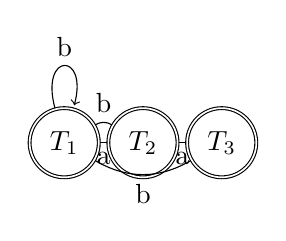
\begin{tikzpicture}
        \node[state, accepting] (t1) {$T_1$};
        \node[state, accepting, right of=t1] (t2) {$T_2$};
        \node[state, accepting, right of=t2] (t3) {$T_3$};
        \draw (t1) edge[below] node{a} (t2)
        (t2) edge[below] node{a} (t3)
        (t3) edge[below, bend left=30] node{b} (t1)
        (t2) edge[above, bend right] node{b} (t1)
        (t1) edge[loop above] node{b} (t1);
    \end{tikzpicture}
\end{document}